% Options for packages loaded elsewhere
\PassOptionsToPackage{unicode}{hyperref}
\PassOptionsToPackage{hyphens}{url}
%
\documentclass[
]{article}
\usepackage{lmodern}
\usepackage{amssymb,amsmath}
\usepackage{ifxetex,ifluatex}
\ifnum 0\ifxetex 1\fi\ifluatex 1\fi=0 % if pdftex
  \usepackage[T1]{fontenc}
  \usepackage[utf8]{inputenc}
  \usepackage{textcomp} % provide euro and other symbols
\else % if luatex or xetex
  \usepackage{unicode-math}
  \defaultfontfeatures{Scale=MatchLowercase}
  \defaultfontfeatures[\rmfamily]{Ligatures=TeX,Scale=1}
\fi
% Use upquote if available, for straight quotes in verbatim environments
\IfFileExists{upquote.sty}{\usepackage{upquote}}{}
\IfFileExists{microtype.sty}{% use microtype if available
  \usepackage[]{microtype}
  \UseMicrotypeSet[protrusion]{basicmath} % disable protrusion for tt fonts
}{}
\makeatletter
\@ifundefined{KOMAClassName}{% if non-KOMA class
  \IfFileExists{parskip.sty}{%
    \usepackage{parskip}
  }{% else
    \setlength{\parindent}{0pt}
    \setlength{\parskip}{6pt plus 2pt minus 1pt}}
}{% if KOMA class
  \KOMAoptions{parskip=half}}
\makeatother
\usepackage{xcolor}
\IfFileExists{xurl.sty}{\usepackage{xurl}}{} % add URL line breaks if available
\IfFileExists{bookmark.sty}{\usepackage{bookmark}}{\usepackage{hyperref}}
\hypersetup{
  pdftitle={Lake Photic Zone Temperature across the Conterminous United States},
  pdfauthor={Kreakie, B. J. * 1, Shivers, S. 2, Hollister. J. W. 1, Milstead, W. Bryan. 1,; 1 US Environmental Protection Agency, Office of Research and Development, Atlantic Coastal Environmental Sciences Division (ACESD), Narragansett, RI 02882; 2 ORISE, Narragansett, RI 02882; * *corresponding author: kreakie.betty@epa.gov*},
  hidelinks,
  pdfcreator={LaTeX via pandoc}}
\urlstyle{same} % disable monospaced font for URLs
\usepackage[margin=1in]{geometry}
\usepackage{graphicx,grffile}
\makeatletter
\def\maxwidth{\ifdim\Gin@nat@width>\linewidth\linewidth\else\Gin@nat@width\fi}
\def\maxheight{\ifdim\Gin@nat@height>\textheight\textheight\else\Gin@nat@height\fi}
\makeatother
% Scale images if necessary, so that they will not overflow the page
% margins by default, and it is still possible to overwrite the defaults
% using explicit options in \includegraphics[width, height, ...]{}
\setkeys{Gin}{width=\maxwidth,height=\maxheight,keepaspectratio}
% Set default figure placement to htbp
\makeatletter
\def\fps@figure{htbp}
\makeatother
\setlength{\emergencystretch}{3em} % prevent overfull lines
\providecommand{\tightlist}{%
  \setlength{\itemsep}{0pt}\setlength{\parskip}{0pt}}
\setcounter{secnumdepth}{-\maxdimen} % remove section numbering

\title{Lake Photic Zone Temperature across the Conterminous United States}
\author{Kreakie, B. J. \textsuperscript{*} \textsuperscript{\emph{1}}, Shivers,
S. \textsuperscript{\emph{2}}, Hollister. J. W.
\textsuperscript{\emph{1}}, Milstead, W. Bryan.
\textsuperscript{\emph{1}}, \and \textsuperscript{\emph{1}} US Environmental Protection Agency, Office of
Research and Development, Atlantic Coastal Environmental Sciences
Division (ACESD), Narragansett, RI 02882 \and \textsuperscript{\emph{2}} ORISE, Narragansett, RI 02882 \and \textsuperscript{*} *corresponding author:
\href{mailto:kreakie.betty@epa.gov*}{\nolinkurl{kreakie.betty@epa.gov*}}}
\date{}

\begin{document}
\maketitle
\begin{abstract}
As the average global air temperature on Earth increases, surface
temperatures of lakes are also increasing globally (0.34 °C per decade
from 1985 to 2009). The influence of this increased temperature touches
all biotic and abiotic components of lentic ecosystems. Here we present
a simple yet robust model of lake photic zone temperature using the 2007
and 2012 US EPA's National Lakes Assessment data for the conterminous
United States. The final model has a mean square error of 2.19 and an
adjusted R(n2) of 0.88. The sampling date, that day's average ambient
air temperature, data obtained from the PRISM Climate Group, and
longitude are the most important variables impacting the final model's
accuracy. Given the importance of temperature to a lake ecosystem,
especially to cyanobacteria bloom dynamics, this model can be a valuable
tool for researchers and lake resource managers. Daily predicted lake
photic zone temperature for all lakes in the conterminous US can now be
straightforwardly estimated based on basic ambient temperature and
location information.
\end{abstract}

\hypertarget{introduction}{%
\section{Introduction}\label{introduction}}

During a time of unprecedented environmental and climatic variability,
lakes can serve as sentinels and integrators in a changing world
{[}1,2{]}. As the average global air temperature on Earth increases
(0.15-0.20 °C per decade since 1975){[}3{]}, surface temperatures of
lakes are also increasing globally (0.34 °C per decade from 1985 to
2009) {[}4{]}. The influence of this increased temperature touches all
biotic and abiotic components of lentic ecosystems. Ultimately,
temperature changes will greatly impact every aspects of lake resource
management. For example, temperature, in addition to nutrients, is a key
driver to cyanobacteria bloom dynamics {[}5{]}. During periods of higher
temperature, cyanobacteria species dominate the phytoplankton community
{[}6--8{]}. As lake temperature increase (typically above 25°C),
cyanobacteria have a competitive advantage over phytoplankton and can
proliferate quickly {[}9{]}. Moreover, experimentally enhanced water
temperatures yielded significantly increased growth rates of higher
toxic Microcystis, but not the non-toxic strains {[}10{]}. Thus, our
ability to understand and predict toxic cyanobacteria blooms will be
deeply dependent on our ability to forecast lake photic zone
temperature. This need for accurate lake temperature forecasting will be
crucial for protecting human and environmental health.

Because to the ecological significance, it is not surprising that
modelling near-surface lake temperature has been broadly investigated.
Models typically vary in number of lakes studied, complexity of
modelling approach, and study interval. Modelling efforts include
efforts to model a single lake predicted over relatively small-time
intervals (like hourly predictions). Such studies include: {[}11--13{]}.
There are numerous studies that model temperature for a small number of
lakes while attempting to limit the number of predictor variables
{[}14--17{]}. By and large, air temperature and lake size are often the
only selected predictor variables. On the whole, very few modelling
efforts attempt to predict lake temperature across large spatial extents
for large number of lakes. Yet some examples include: {[}4,19,20{]}.
Despite this great variation in approach and execution, most have been
rather successful modelling lake photic zone temperature, although it is
important to note that the majority of these lakes are large.
Considering that the number and importance of small lakes (\textless{}
1km2) has been historically underestimated, it is important to also
predict temperatures in these small lakes {[}21,22{]}.

In summary, we still lack the ability to robustly model near-surface
temperature for all lakes across a large spatial extent. Modelling lake
temperature requires a large amount of data, and therefore study lakes
are often selected opportunistically, which may introduce a spatial
bias. Frequently, the study lakes have a high regional resource value
(e.g.~the Great Lakes) and commonly have an extensive monitoring history
due to the vested interest of the public. When model efforts do attempt
to cross large spatial extents, these efforts often rely on satellite
data. While these models predict over large areas, they are restricted
by the size of the lake captured by satellite (typically 3km2 for 1 km
MODIS pixels).

The presented modelling effort uses the US Environmental Protection
Agency's (EPA's) National Lake Assessment (NLA). The NLA is a stratified
random sample of all lakes in the conterminous United States repeated
every five years beginning in 2007. Even though this is a large effort
involving numerous agencies, the sampling methods are standardized and
have a comprehensive quality assurance plan. The uniqueness of this data
set allows us to build a robust lake photic zone temperature model for
all US lakes. By using lakes across the US (i.e.~at a large spatial
extent), we included lakes with different morphologies, in different
climates with diverse geologies, and surrounding landscapes.
Additionally, small lakes were well represented with more than 50\% of
the lakes in the 2012 survey less than 0.5 km2.

To summarize, the main goal of this work was to develop a simple yet
robust lake photic temperature model for all lakes in the conterminous
US that capture key drivers of near-surface lake temperature.
Additionally, this work (something about open science and GitHub link).

\hypertarget{methods}{%
\section{Methods}\label{methods}}

\#\#Data We relied on the in situ temperature data provided in the US
EPA's National Lake Assessment (NLA) (CITE). The NLA is a stratified
random sample of lakes (great than 1 ha) across the United States. NLA
sampling took place in 2007, 2012, and 2017. This research effort used
the 2007 and 2012 sample years. The 2017 data are currently undergoing
quality control before being released the public. Upon release, the data
can easily be included to improve this model. For both sample years, we
have included over 1,000 lakes across the conterminous US excluding the
Great Lakes (Figure 1). For each sampled lake, we used the mean
temperature for all sampled depths of less than 2m (this being the depth
typically considered the photic zone).

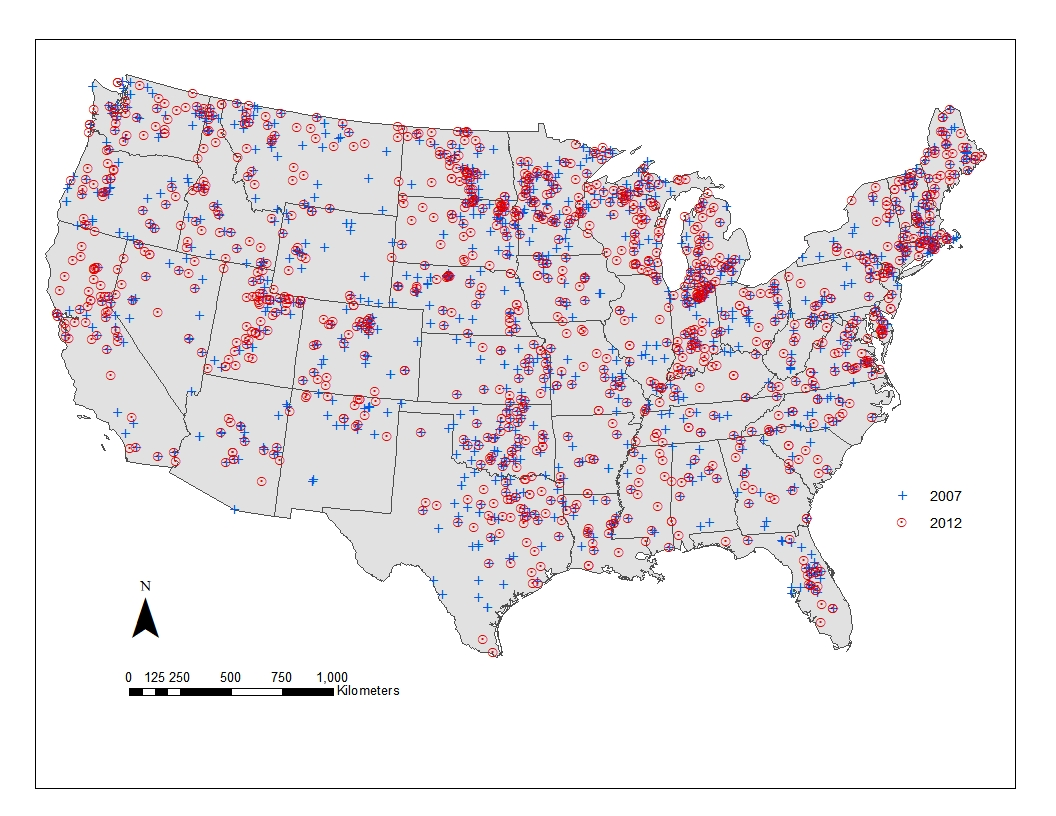
\includegraphics{../figures/LakePhoticZonev2.jpg} Figure 1: Map of 2007
and 2012 US EPA's National Lake Assessment (NLA) Lakes

We included numerous predictor variables that are hypothesized to impact
lake photic zone. As a proxy for directly measured ambient air
temperature, we used the PRISM AN81d dataset (PRISM Climate Group,
Oregon State University, \url{http://prism.oregonstate.edu}, created 07
Nov 2018). This dataset provides interpolated daily temperature
estimates (mean, maximum, and minimum) for 4km grids in the conterminous
United States for 1981 to the present (see:
\url{http://www.prism.oregonstate.edu/documents/PRISM_datasets.pdf}).
PRISM takes advantage of measured climate variables to interpolate point
data to spatially defined grids using regression techniques and expert
knowledge (Daly et al 2008). For our study, we used the ``prism'' R
package (Hart \& Bell) to download the mean daily temperatures for the
PRISM grid cells corresponding to the centroids of all NLA lakes
included in this study for dates between 01 May and 30 September of 2007
and 2012.

In addition to climate, there are additional factors clearly impacting
lake temperature (e.g., surrounding land use, lake depth, size, and
configuration, and elevation). To test for the relative importance of
lake morphometry and surrounding landscape, we used the R packages
\texttt{lakemorpho} to calculate a suite of lake morphometry metric and
\texttt{elevatr} to access digital elevation models for each lake
{[}23,24{]}. Additionally, National Land Cover Database (NLCD) was our
source for landcover data. Specifically, we calculated the percent
impervious surface of a 3000m buffer for each lake. Lakes with partials
buffers falling outside the US were excluded.

To test the relative influence of both short and long-term temperature,
we derived several measures for a lake's local air temperature. Mean air
temperatures for day of and the day before the sample date were
extracted directly from the prism data. To understand longer term
influences we calculated average mean air temperatures for periods 3, 7,
and 30 days prior to the sample date.

\hypertarget{random-forest-modelling}{%
\subsection{Random Forest Modelling}\label{random-forest-modelling}}

Random forest modelling was used to not only develop a predictive model
of photic zone temperature, but also used as a means of variable
selection and calculate relative variable importance. Random forest is a
machine learning method that builds a consensus prediction from the
assemblage of multiple tree models (here specifically 10,000 trees for
the final model and 1,000 trees for the variable selection models). Each
individual tree model is constructed from a subset of the full data set
and a subset of all predictor variables.All random forest modelling was
conducted in R v XXXX (CITE) with the randomForest package (CITE). Model
performance is reported as mean square error and adjusted R.

Random forest does not require that users reduce the number of predictor
variables; the random forest algorithm prevents overfitting and is not
impacted by correlated predictor variables (Culter 2007). While it is
unlikely that random forest models constructed with reduced numbers of
predictor variables perform any better than models constructed with a
full suite of available variables(Fox et al., 2017), reducing the number
of our predictor variables was necessary in order to fulfill the
long-term goals of this work. Several of our climatic predictor
variables are computationally intensive to create for the entire
conterminous United States. In order to use our final model for future
forecasting or historical backcasting, we strove to create a robust
predictive model while minimizing computational demands. To determine
the optimal number and set of variables, we followed the variable
selection method presented in (Hollister 2016).

In addition to measure of overall model performance, we used percent
increase of mean-squared error to assess variable importance. The
percent increase in mean-squared error is a comparison between the true
values of a variable and randomly permuted values of a specific variable
on overall model performance.

\hypertarget{results}{%
\section{Results}\label{results}}

We used 1185 data points from the 2007 NLA and 1097 from 2012 NLA.
Figure 1 illustrates the spatial distribution of the sampled lakes.

Figure 1

Using the average temperature for the upper two meters as the response
variable, we initially began the variable selection process with 16
predictor variables. The variable selection process identified a reduced
model with 7 variables (Figure 2). The selected variables were average
ambient air temperature for the sample date, sample date, longitude,
average ambient air temperature for 30 day proceeding the sample date,
elevation, latitude, length of lake shoreline, and the lake surface
area.

\begin{figure}
\centering
\includegraphics{../figures/varselfig.jpg}
\caption{Figure 2: Variable selection plot for all variables. Shows
percent increase in mean square error as a function of the number of
variables.}
\end{figure}

The final model built with the eight selected variables has a
mean-squared error of 2.19 and adjusted R(n2) of 0.88. The variables
ranked in order of importance were date, average temperature, longitude,
30-day average temperature, elevation, latitude, surface area, and
shoreline length (Figure 3). The partial dependency plots illustrate how
the predicted photic zone temperature changes over the range of values
for all predictor variables (Figure 4).

\begin{figure}
\centering
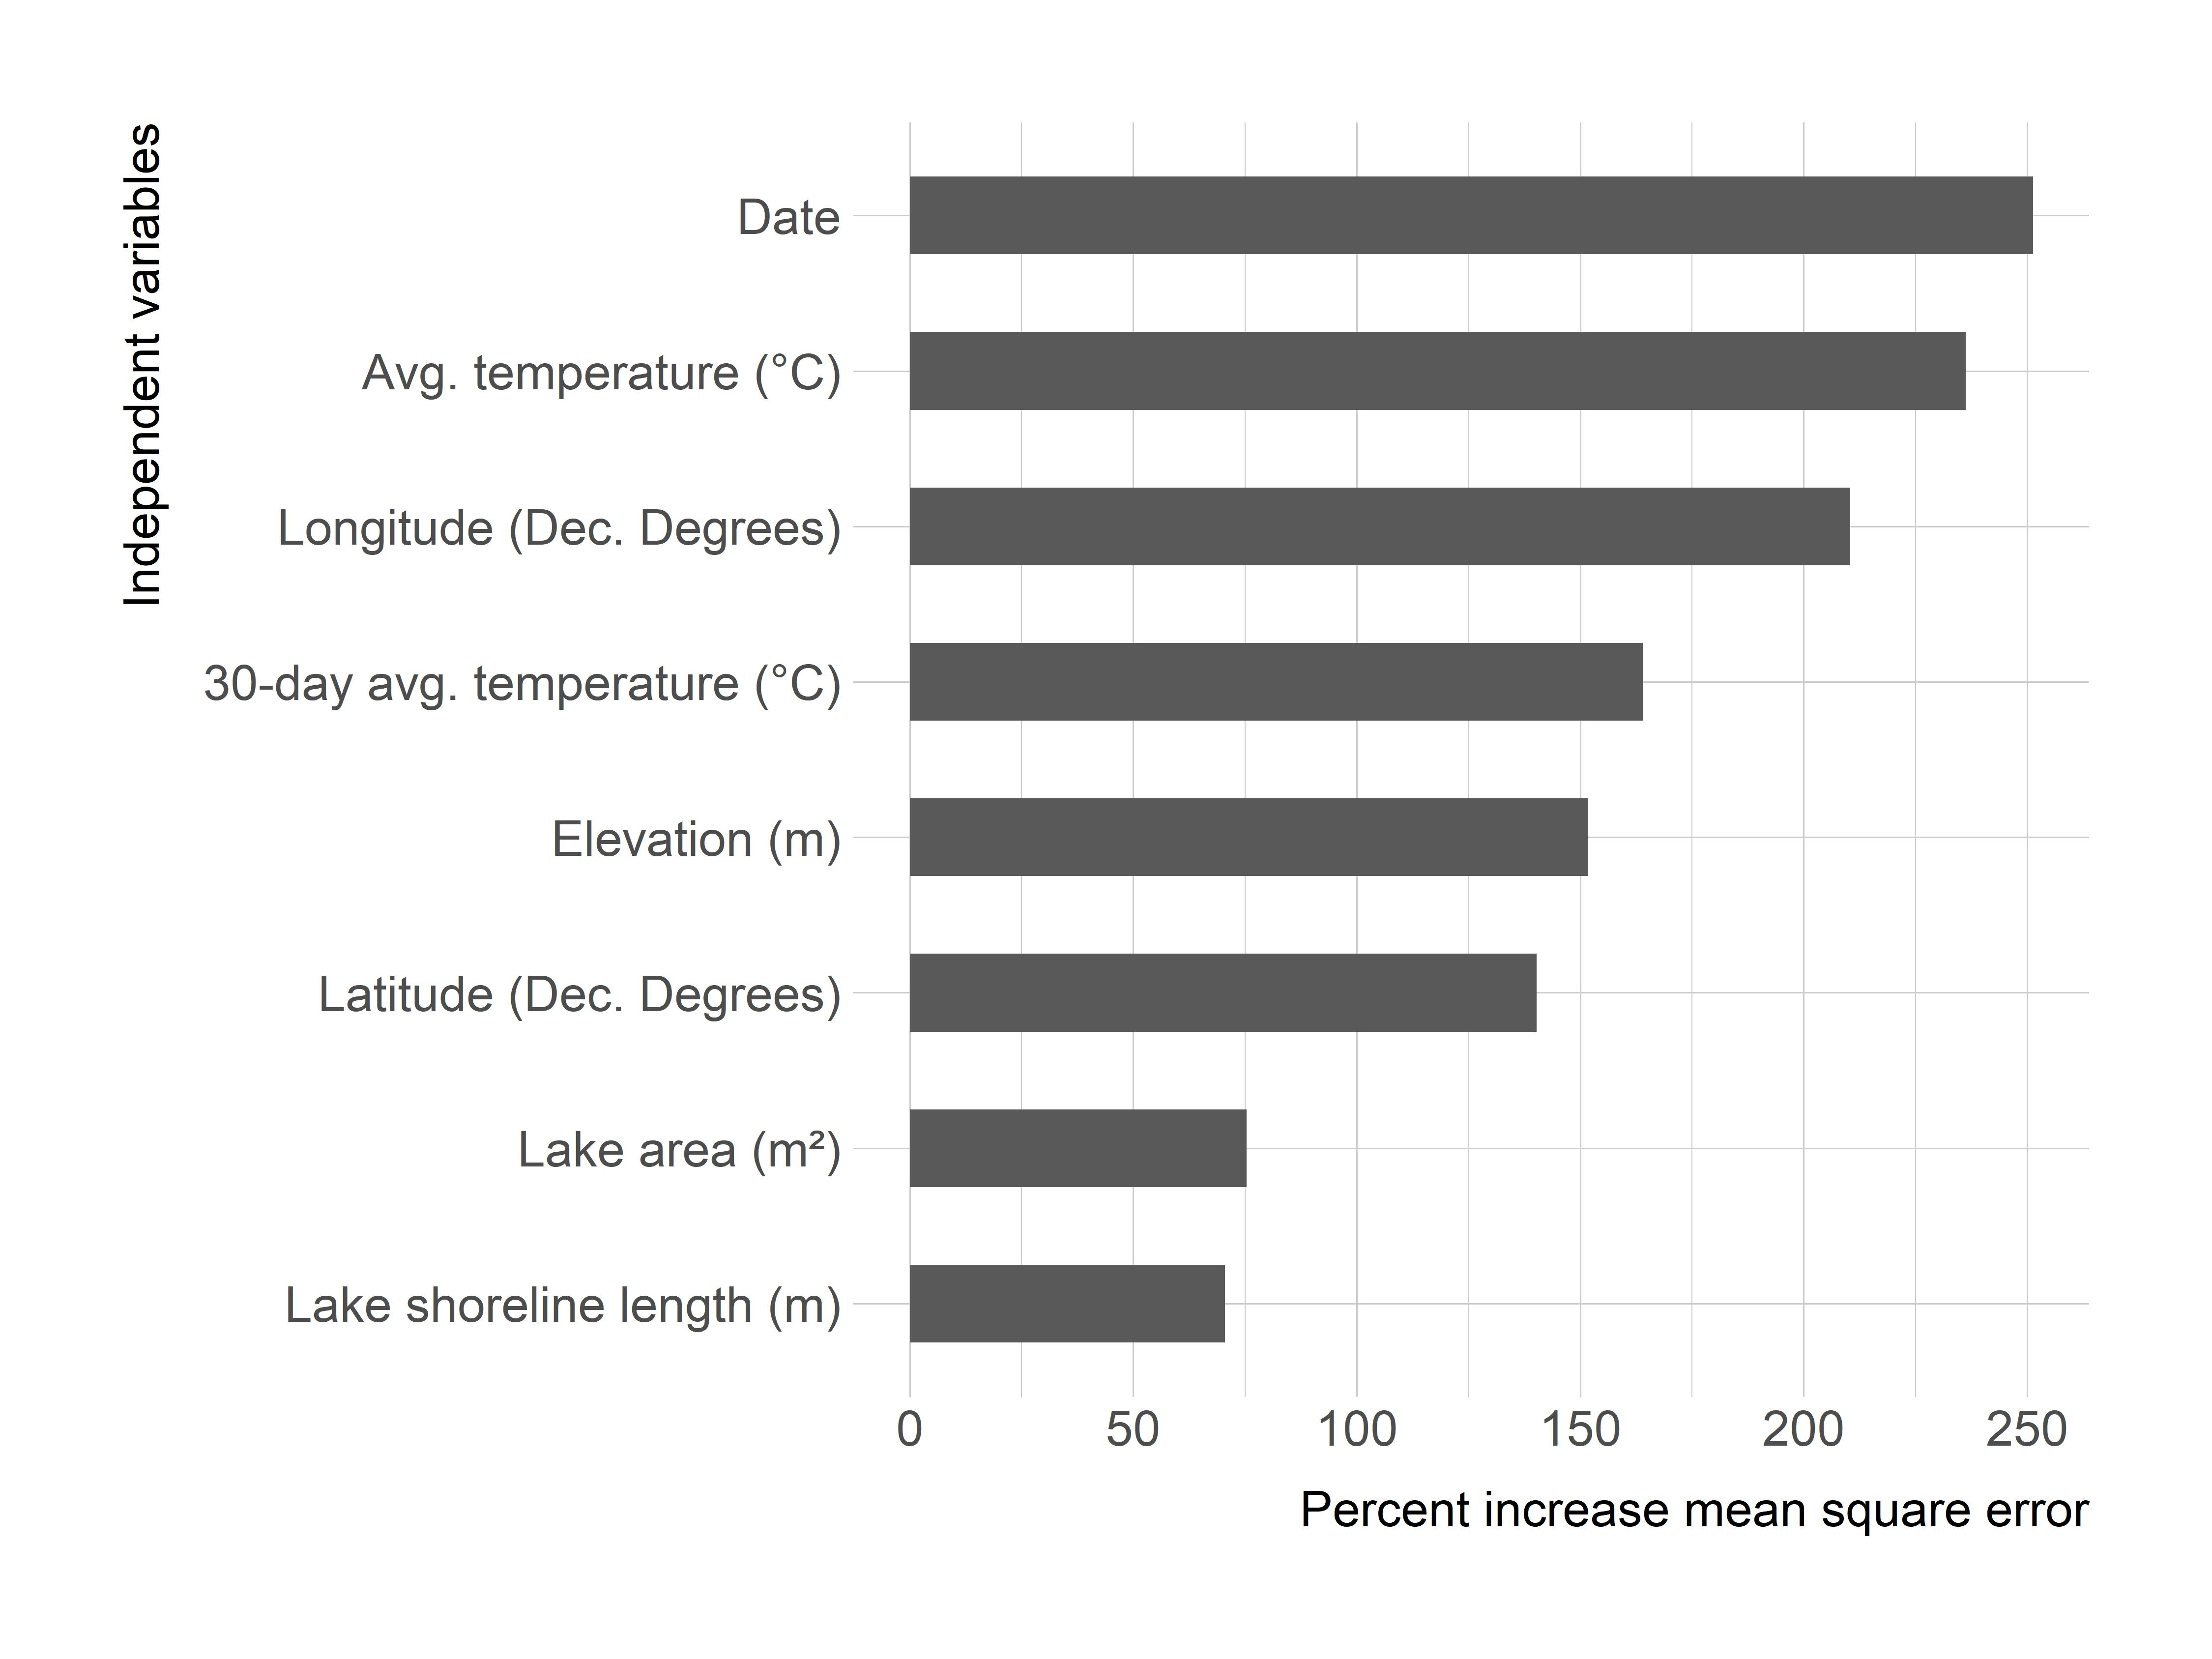
\includegraphics{../figures/varImpPlot.jpg}
\caption{Figure 3: Variable importance plot for selected variables.
Shows precent increase in mean square error. Higher values indicate a
higher impact on overall model accuracy.}
\end{figure}

\begin{figure}
\centering
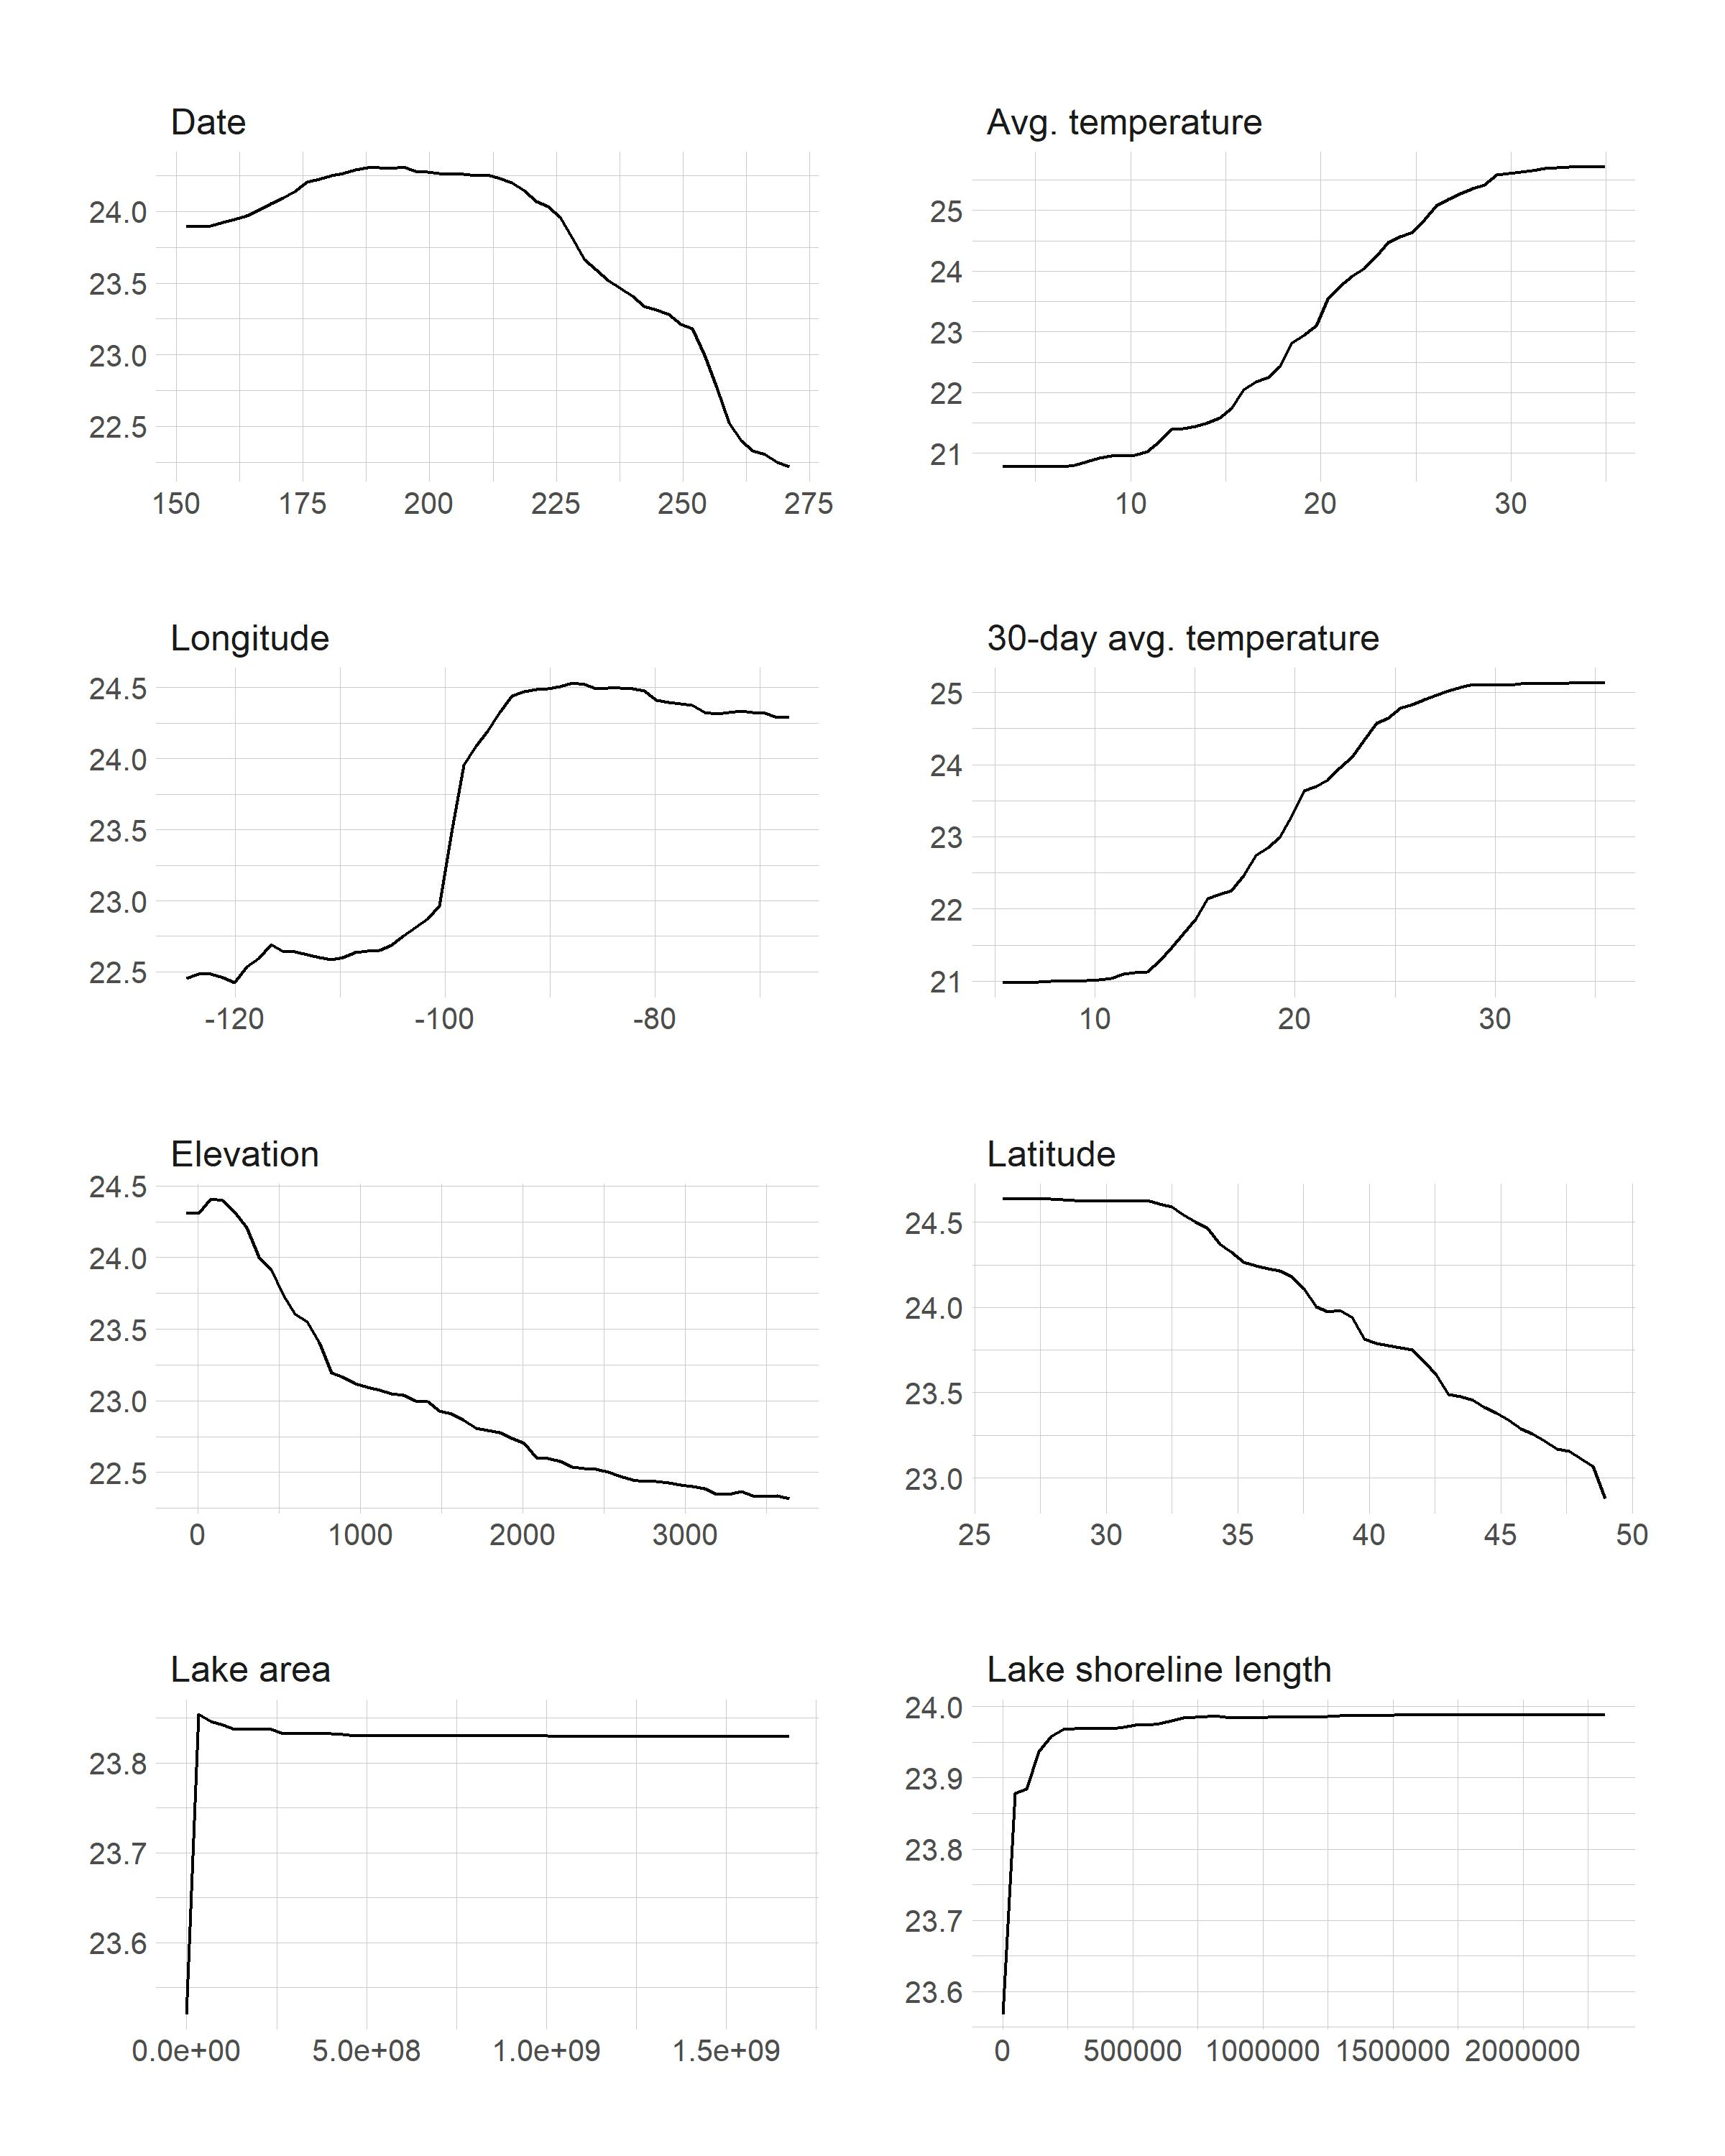
\includegraphics{../figures/partPlot.jpg}
\caption{Figure 4: Partial dependence plots for selected variables.}
\end{figure}

\hypertarget{discussion-and-conclusions}{%
\section{Discussion and conclusions}\label{discussion-and-conclusions}}

Here we present a simple yet robust model of lake photic zone
temperature using the 2007 and 2012 NLA data for the conterminous United
States. The final model has a mean square error of 2.19 and an adjusted
R(n2) of 0.88. The sampling date, that day's average ambient air
temperature, data obtained from the PRISM Climate Group, and longitude
are the most important variables impacting the final model's accuracy.
Given the importance of temperature to a lake ecosystem, especially to
cyanobacteria bloom dynamics, this model can be a valuable tool for
researchers and lake resource managers. Daily predicted lake photic zone
temperature for all lakes in the conterminous US can now be
straightforwardly estimated based on basic ambient temperature and
location information.

Using only easily obtainable metrics to estimate lake temperature was a
primary focus in the creation of this model. Several studies
(e.g.~{[}25{]}) have used similar metrics with good results (RMSE=0.5
°C) to estimate lake temperature but were applied to a single, or a
small number of lakes. Other studies have used more complex models
(e.g.~GLM) to yield good results (RMSE = 1.62 °C for the epilimnion) at
varying scales {[}26,27{]}. However, these models require more complex
input variables which are not available for all lakes and may be biased
towards large lakes. Using the NLA data and simple metrics allowed this
model to be applicable to any lake within the conterminous United States
using minimal input data with a small increase in RMSE. Additionally,
this model is predictive and the model and data will be made publicly
available.

The final model included, average ambient air temperature and the
average temperature of the prior 30 days. Yet the 3-day and 7-day prior
to the sampling date averages were not selected in the final model. It
is likely that the three and seven day averages are not providing the
model with unique information. Typical the three and seven day averages
are fairly close the day-of average. Ambient air temperature does not
change drastically over such a short time scale. Even if a big swing in
temperature did happen during this short time period, it would be too
rare to be a significant factor in the model. Yet the longer term 30-day
average does have an impact on lake photic zone temperature. The 30-day
average provides us with this information about the temperature
intensity leading up to the sample date. Not just how far along into
summer; that information would be captured in the date parameter. But
more specifically, this measures the long term thermal heating happening
at a site.

In addition to the several derived air temperature variables, we
included land-use/land cover variables in our initial variable selection
process. Specifically, we calculated the percent impervious surface for
a 3km lake buffer and a measure of shoreline development. These
variables were included based on the hypothesis that higher amounts of
development and therefore impervious surface surrounding a lake would
lead to higher temperatures in lakes. Yet neither of these variables
were selected in the final model. Even though the land-use variables
were not selected that does not mean development and impervious are not
impactful. This urban-heat effect on lakes may have been adequately
captured in the average ambient air temperature. Therefore, making the
land-use variables redundant. Regardless these variables did not
independently contribute to the model's accuracy.

Despite being one of the most common measurements collected by
limnologists, lake temperature datasets that cover long periods of time
are very difficult to obtain. Sharma et al (2015) have compiled summer
lake temperature data for 291 lakes for the period 1985-2009. This may
be the largest lake temperature database to date, however, the data are
only available to members of their research group and, realistically,
the number of lakes included is very small. One of the reasons we chose
to model lake photic zone temperature was to develop a database of lake
temperatures for the 48 conterminous United States. The model we present
has proven to be accurate and will allow us to backcast lake
temperatures for all the \textgreater{} 300,000 lakes included in
NHDplus for the period of time covered by the PRISM climate predictions
(1981 to present). This dataset will allow us to investigate how photic
zone temperatures vary both spatially and temporally across the United
States. This database is being developed and, when complete, will be
made available as an open source data set.

\hypertarget{bibliography}{%
\section*{Bibliography}\label{bibliography}}
\addcontentsline{toc}{section}{Bibliography}

\hypertarget{refs}{}
\leavevmode\hypertarget{ref-williamson2009lakes}{}%
1. Williamson CE, Saros JE, Vincent WF, Smol JP (2009) Lakes and
reservoirs as sentinels, integrators, and regulators of climate change.
Limnology and Oceanography 54: 2273--2282.

\leavevmode\hypertarget{ref-schindler2009lakes}{}%
2. Schindler D (2009) Lakes as sentinels and integrators for the effects
of climate change on watersheds, airsheds, and landscapes. Limnology and
Oceanography 54: 2349--2358.

\leavevmode\hypertarget{ref-hansen2010global}{}%
3. Hansen J, Ruedy R, Sato M, Lo K (2010) Global surface temperature
change. Reviews of Geophysics 48.

\leavevmode\hypertarget{ref-o2015rapid}{}%
4. O'Reilly CM, Sharma S, Gray DK, Hampton SE, Read JS, et al. (2015)
Rapid and highly variable warming of lake surface waters around the
globe. Geophysical Research Letters 42: 10--773.

\leavevmode\hypertarget{ref-paerl2012climate}{}%
5. Paerl HW, Paul VJ (2012) Climate change: Links to global expansion of
harmful cyanobacteria. Water research 46: 1349--1363.

\leavevmode\hypertarget{ref-lurling2013comparison}{}%
6. Lürling M, Eshetu F, Faassen EJ, Kosten S, Huszar VL (2013)
Comparison of cyanobacterial and green algal growth rates at different
temperatures. Freshwater Biology 58: 552--559.

\leavevmode\hypertarget{ref-o2012rise}{}%
7. O'neil J, Davis T, Burford M, Gobler C (2012) The rise of harmful
cyanobacteria blooms: The potential roles of eutrophication and climate
change. Harmful algae 14: 313--334.

\leavevmode\hypertarget{ref-peperzak2003climate}{}%
8. Peperzak L (2003) Climate change and harmful algal blooms in the
north sea. Acta Oecologica 24: S139--S144.

\leavevmode\hypertarget{ref-paerl2008blooms}{}%
9. Paerl HW, Huisman J (2008) Blooms like it hot. Science 320: 57--58.

\leavevmode\hypertarget{ref-davis2009effects}{}%
10. Davis TW, Berry DL, Boyer GL, Gobler CJ (2009) The effects of
temperature and nutrients on the growth and dynamics of toxic and
non-toxic strains of microcystis during cyanobacteria blooms. Harmful
algae 8: 715--725.

\leavevmode\hypertarget{ref-saeed2016water}{}%
11. Saeed S, Honeyeh K, Ozgur K, Wen-Cheng L (2016) Water temperature
prediction in a subtropical subalpine lake using soft computing
techniques. Earth Sciences Research Journal 20: 1--11.

\leavevmode\hypertarget{ref-peeters2002modeling}{}%
12. Peeters F, Livingstone DM, Goudsmit G-H, Kipfer R, Forster R (2002)
Modeling 50 years of historical temperature profiles in a large central
european lake. Limnology and Oceanography 47: 186--197.

\leavevmode\hypertarget{ref-zhong2016recent}{}%
13. Zhong Y, Notaro M, Vavrus SJ, Foster MJ (2016) Recent accelerated
warming of the laurentian great lakes: Physical drivers. Limnology and
Oceanography 61: 1762--1786.

\leavevmode\hypertarget{ref-matuszek1996empirical}{}%
14. Matuszek JE, Shuter BJ (1996) An empirical method for the prediction
of daily water temperatures in the littoral zone of temperate lakes.
Transactions of the American Fisheries Society 125: 622--627.

\leavevmode\hypertarget{ref-kettle2004empirical}{}%
15. Kettle H, Thompson R, Anderson NJ, Livingstone DM (2004) Empirical
modeling of summer lake surface temperatures in southwest greenland.
Limnology and Oceanography 49: 271--282.

\leavevmode\hypertarget{ref-piccolroaz2016prediction}{}%
16. Piccolroaz S (2016) Prediction of lake surface temperature using the
air2water model: Guidelines, challenges, and future perspectives.
Advances in Oceanography and Limnology.

\leavevmode\hypertarget{ref-toffolon2014prediction}{}%
17. Toffolon M, Piccolroaz S, Majone B, Soja A-M, Peeters F, et al.
(2014) Prediction of surface temperature in lakes with different
morphology using air temperature. Limnology and Oceanography 59:
2185--2202.

\leavevmode\hypertarget{ref-livingstone1998relationship}{}%
18. Livingstone DM, Lotter AF (1998) The relationship between air and
water temperatures in lakes of the swiss plateau: A case study with
pal\(\backslash\)sgmaelig; olimnological implications. Journal of
Paleolimnology 19: 181--198.

\leavevmode\hypertarget{ref-minns2017factors}{}%
19. Minns CK, Shuter BJ, Davidson A, Wang S (2017) Factors influencing
peak summer surface water temperature in canada's large lakes. Canadian
Journal of Fisheries and Aquatic Sciences 75: 1005--1018.

\leavevmode\hypertarget{ref-wan2017comprehensive}{}%
20. Wan W, Li H, Xie H, Hong Y, Long D, et al. (2017) A comprehensive
data set of lake surface water temperature over the tibetan plateau
derived from modis lst products 2001--2015. Scientific data 4: 170095.

\leavevmode\hypertarget{ref-downing2006global}{}%
21. Downing JA, Prairie Y, Cole J, Duarte C, Tranvik L, et al. (2006)
The global abundance and size distribution of lakes, ponds, and
impoundments. Limnology and Oceanography 51: 2388--2397.

\leavevmode\hypertarget{ref-winslow2014lake}{}%
22. Winslow LA, Read JS, Hanson PC, Stanley EH (2014) Lake shoreline in
the contiguous united states: Quantity, distribution and sensitivity to
observation resolution. Freshwater biology 59: 213--223.

\leavevmode\hypertarget{ref-hollister2017lakemorpho}{}%
23. Hollister J, Stachelek J (2017) Lakemorpho: Calculating lake
morphometry metrics in r. F1000Research 6.

\leavevmode\hypertarget{ref-hollister2017elevatr}{}%
24. Hollister J, Tarak Shah (2017) Elevatr: Access elevation data from
various apis. Available: \url{http://github.com/usepa/elevatr}.

\leavevmode\hypertarget{ref-piccolroaz2018predictability}{}%
25. Piccolroaz S, Healey N, Lenters J, Schladow S, Hook S, et al. (2018)
On the predictability of lake surface temperature using air temperature
in a changing climate: A case study for lake tahoe (usa). Limnology and
Oceanography 63: 243--261.

\leavevmode\hypertarget{ref-bruce2018multi}{}%
26. Bruce LC, Frassl MA, Arhonditsis GB, Gal G, Hamilton DP, et al.
(2018) A multi-lake comparative analysis of the general lake model
(glm): Stress-testing across a global observatory network. Environmental
Modelling \& Software 102: 274--291.

\leavevmode\hypertarget{ref-hipsey2019general}{}%
27. Hipsey MR, Bruce LC, Boon C, Busch B, Carey CC, et al. (2019) A
general lake model (glm 3.0) for linking with high-frequency sensor data
from the global lake ecological observatory network (gleon).

\end{document}
